\section{Definitionen \& Formate}
Beschreibung der wichtigsten Codex und Datei-Formate, die während des Projektes zum Einsatz kamen.

%%%%%%%%%%%%%%%%%%%%%%%%%%%%%%%%%%%%%%%%%%%%%%%%%%%%%%%%%%%%%%%%%%%%%%%%%%%%%%%
\subsection{webm}
\color{red}
..

\textbf{WIKIpedia - rewrite - Zusammenfassen}
Achtung, kann auch direkt auf einer Website dargestellt werden!\\

Ogg ist ein Container-Dateiformat für Multimedia-Dateien, kann also gleichzeitig Audio-, Video- sowie Textdaten enthalten. Ogg wurde mit dem Ziel konzipiert, eine freie und von Softwarepatenten unbeschränkte Alternative zu proprietären Formaten zu bieten, um Multimedia-Inhalte effizient zu speichern und zu streamen. Die Streamingfähigkeit ist dabei das entscheidende Designmerkmal: Alles, was in einem Ogg-Container verpackt ist, kann ohne zusätzliche Anpassungen gestreamt werden. Dies unterscheidet Ogg von Formaten, die entweder nur in bestimmten Ausprägungen streamingfähig sind (wie z. B. Matroska) oder überhaupt nicht live-streaming-fähig sind (wie z. B. MP4). Ogg-Streams können dabei gebündelt und verkettet werden, ohne dass dazu eine Anpassung des einzelnen Streams notwendig ist.[

Die Entwicklung des Container-Formats wird von der Xiph.Org Foundation geleitet, die auch für einige Codecs verantwortlich ist, welche die Inhalte in einem Ogg-Container komprimieren.

Der bekannteste Codec ist dabei der Audio-Codec Vorbis, welcher oft vereinfachend (oder auch irrtümlich) als Ogg bezeichnet wird, obwohl Ogg tatsächlich nur das Containerformat für die Vorbis-kodierten Inhalte ist. In jüngerer Vergangenheit (seit 2012) setzt sich auch das Vorbis-Nachfolgeformat Opus langsam durch, insbesondere auch im professionellen Broadcast-Umfeld in Hardware-Audio-Codecs. 
\color{black}

Html5 Snippet von www.w3Schools.com zur Anzeige von webm und ogg.
\begin{verbatim}
<video width="320" height="240" controls>
  <source src="movie.webm" type="video/webm">
  Your browser does not support the video tag.
</video> 
\end{verbatim}


%%%%%%%%%%%%%%%%%%%%%%%%%%%%%%%%%%%%%%%%%%%%%%%%%%%%%%%%%%%%%%%%%%%%%%%%%%%%%%%
\subsection{h264}
\color{red}
H.264 ist ein Standard zur Kompression von Videodaten.  \\
\color{black}

\begin{minipage}{\textwidth}
    \begin{center}
        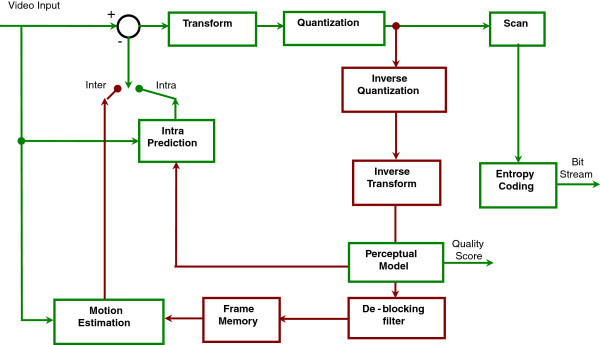
\includegraphics[scale=3.0]{img/h264.jpg} 
    \end{center}
\end{minipage}\\


\section{Vergleich der Streaming-Lösungen und Tests} \label{RefVergleich}
Die Ergebnisse der Versuche wurden übersichtlich in Tabelle 1 zusammengefasst. Von den Ergebnissen ausgehend, wurde die gstreamer Bibliothek für das Streaming vom emb. System ausgewählt und ffmpeg für das zurückstreamen. Gstreamer schien ungeeignet für das zurückstreamen zu sein, da die CPU Leistung des emb. Systems nicht ausreichte, um die Frames auszupacken. Selbst unkomprimierte RAW Frames konnten nicht die Anforderung erfüllen, siehe gstreamer Kapitel \ref{RefGstreamer}.

\begin{table}[H]
\centering
 \begin{tabular}{l|c|c|c}
 \textbf{Streamingtest}&\textbf{Audiodelay [s]}&\textbf{Videodelay [s]} & \textbf{CPU [\%]}\\
\cline{1-4} 
 (a) Testaudio gstreamer PC an localhost          & instant   & --    & --\\
 (b) Testaudio gstreamer emb. System an localhost & instant   & --    & emb.3\\
 (c) Testbild gstreamer PC an localhost           & --        & instant & -- \\
 (d) Testbild gstreamer emb. System an localhost  & --        & instant & emb.20 \\                        
 (e) Audio gstreamer PC an localhost              & instant   & --    & x\\
 (f) Audio gstreamer emb. System an localhost     & instant   & --    & x\\
 (g) Video gstreamer PC an localhost              & --        & 0.1   &  \\
 (h) A/V gstreamer emb.Sys an PC                  & 0.1       & 0.1   & emb.30 \\
 (i) A/V gstreamer PC an emb.System               & ? 20+     & ? 20+ & emb.100\\ 
 \cline{1-4}
 (j) Audio PC ffmpeg - ffplay (localhost)            & 0.2   & --   & --  \\
 (k) Audio PC ffmpeg - ffserver - ffplay (localhost) & 0.4   & --   & --  \\
 (l) Video PC ffmpeg - ffserver - ffplay (localhost) & --    & 1.4  & -- \\
 (m) A/V emb.Sys.- PC ffserver - ffplay              & >2.5  & > 2.5 & emb.30 \\
 (n) A/V PC ffmpeg - ffserver zu emb.Sys. ffplay     & 1.5    & 1.5  & emb.100 \\
\end{tabular}

     \caption{Streaming Delayzeiten}
     \label{tbl:beispieltabelle}
     % Verweis im Text mittels \ref{tbl:beispieltabelle}
   \end{table}

%%%%%%%%%%%%%%%%%%%%%%%%%%%%%%%%%%%%%%%%%%%%%%%%%%%%%%%%%%%%%%%%%%%%%%%%%%%%%%%
\newpage
\section{Anhang: Werbeblatt Jolandi Workerbot4} \label{RefAnhang}
Werbeprospekt für den Service Roboter Jolandi auf zwei Seiten.\\

   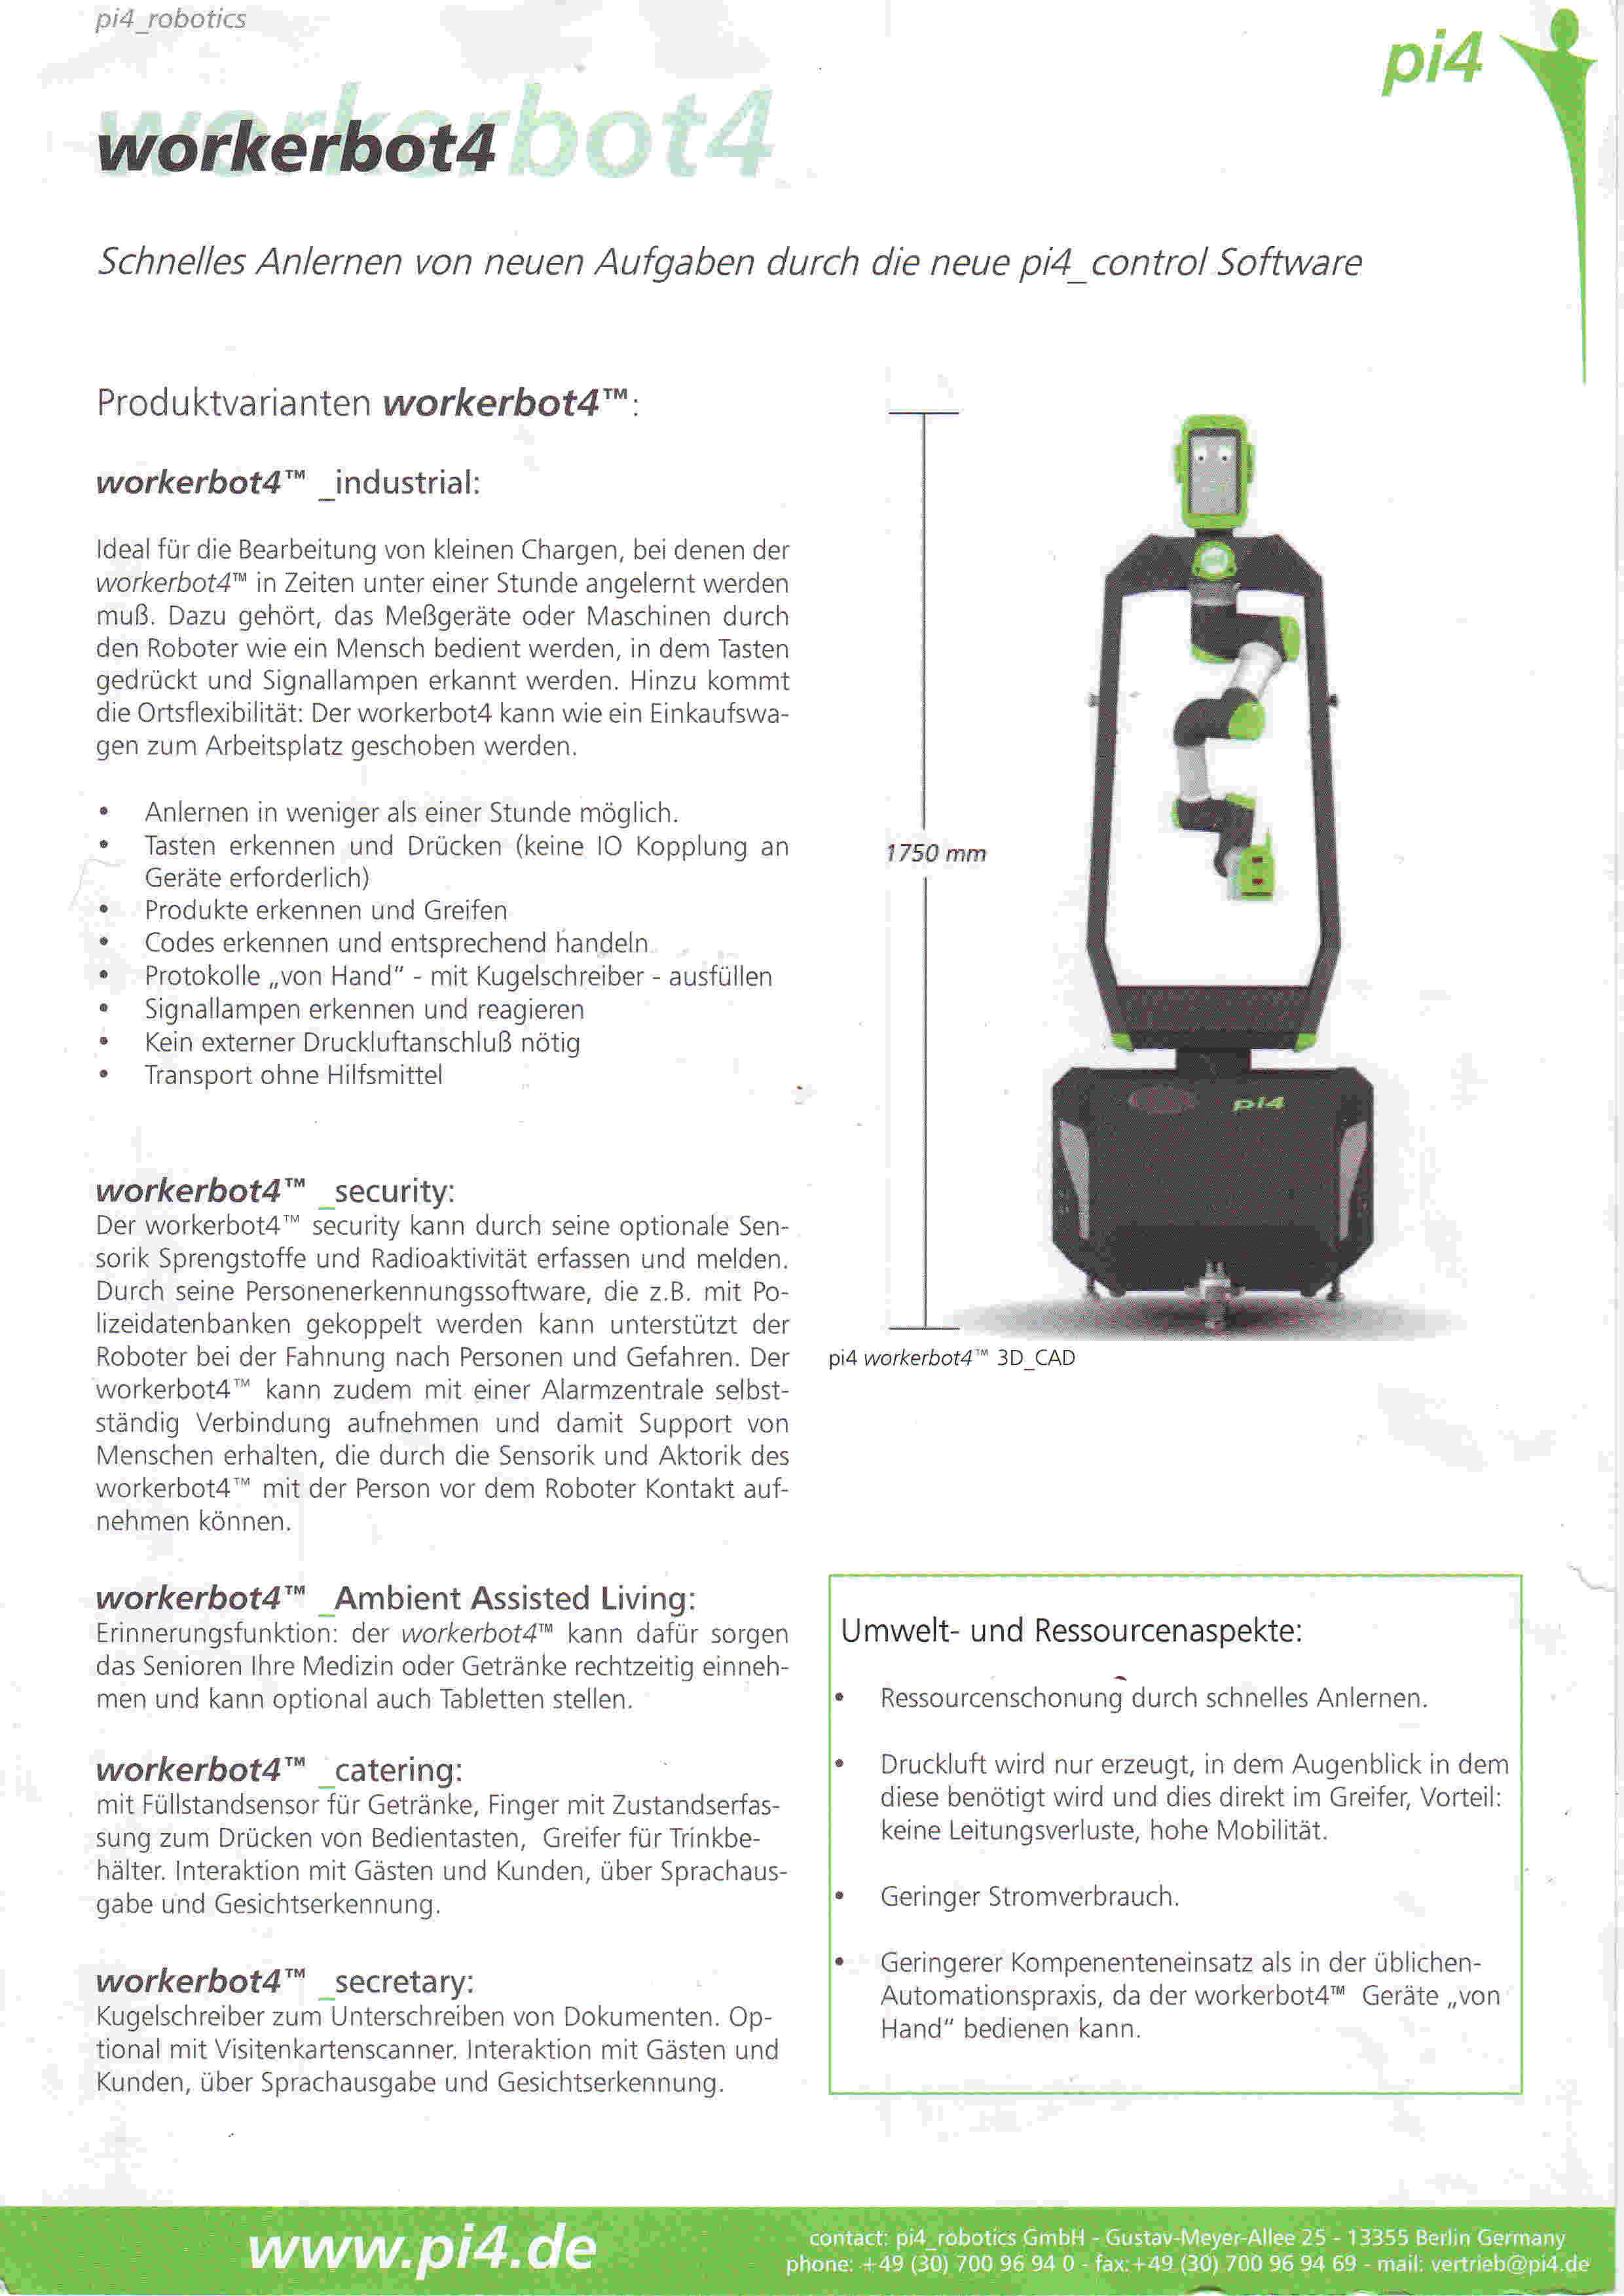
\includegraphics[scale=0.75]{img/jolandi1.jpg} 
   
   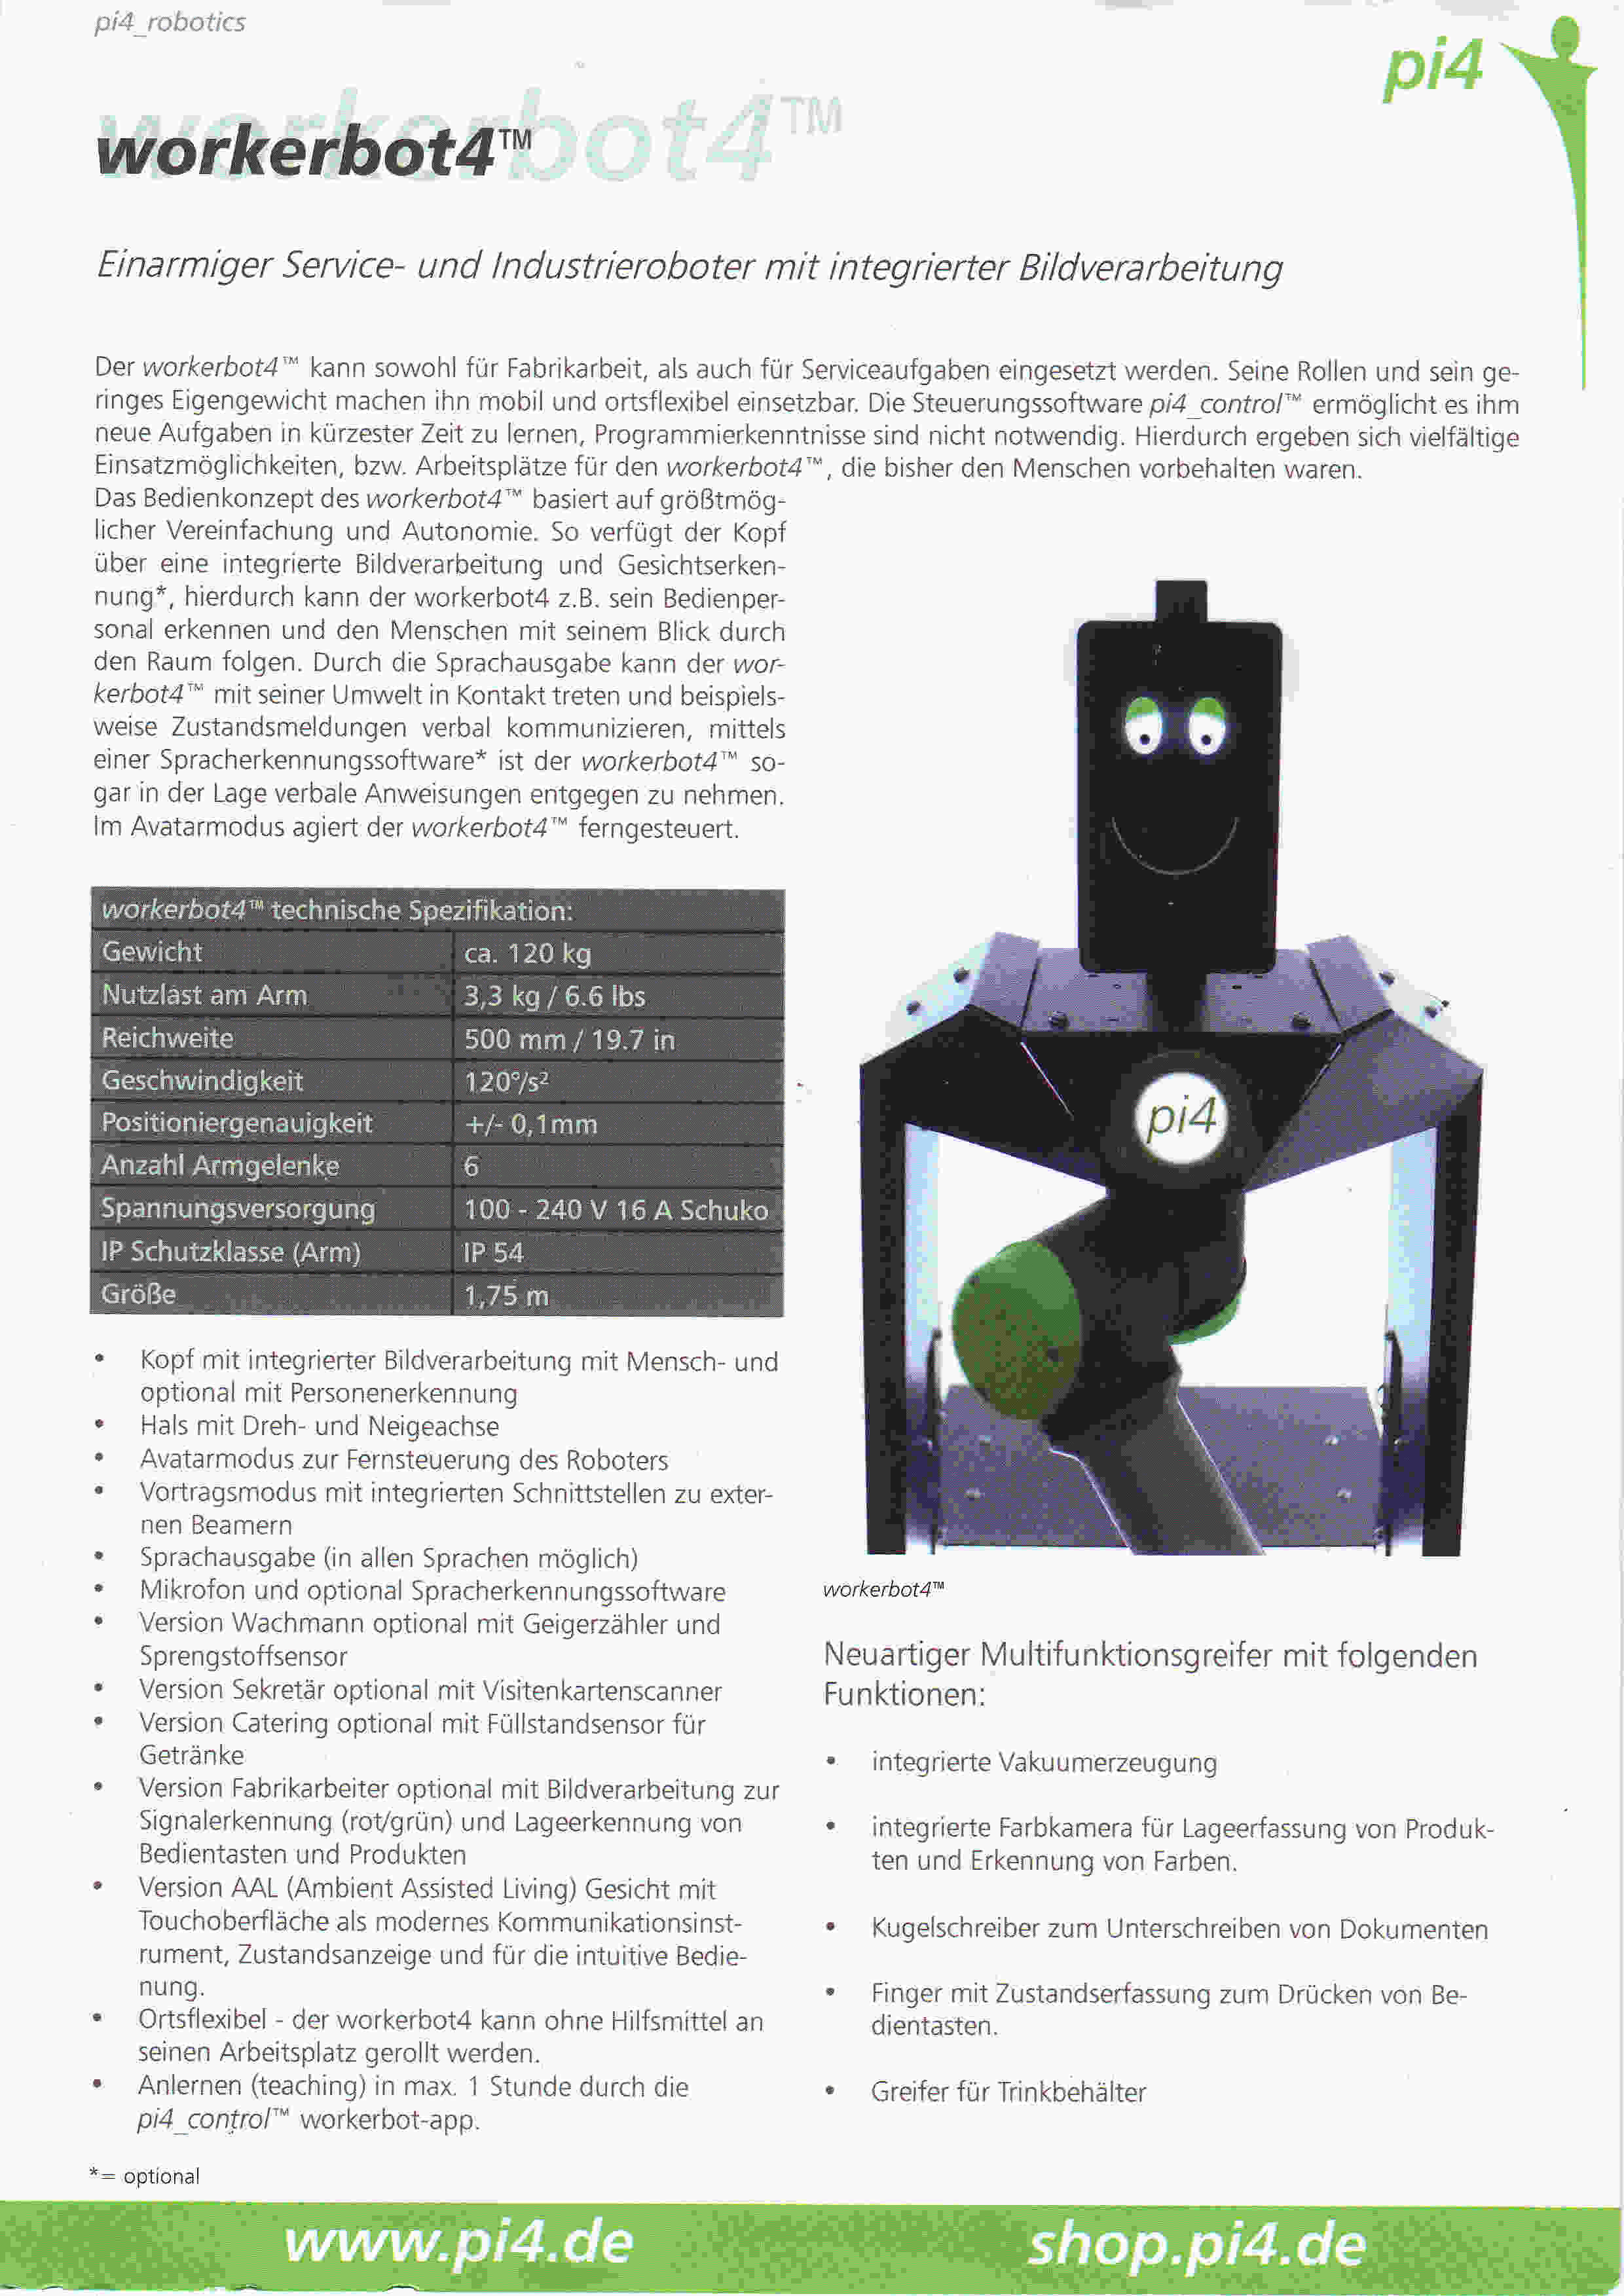
\includegraphics[scale=0.75]{img/jolandi2.jpg} 


